\documentclass[titlepage]{article}
\usepackage{graphicx}
\usepackage{fancyhdr}
\usepackage{tikz}
\pagestyle{fancy}
\fancyhead[L]{\thepage}
\title{\huge Computer Workshop\\Final Assignment}
\author{Morteza Javadian\\ID: 402521162}
\date{Date: 4 Bahman, 1402}

\begin{document}
	
	\maketitle
	
	\renewcommand{\contentsname }{ TABLE OF CONTENTS}
	
	\tableofcontents
	\addtocontents{toc}{~\hfill  Page\par}
	\let\LaTeXStandardTableOfContents\tableofcontents
	
	\renewcommand{\tableofcontents}
	{
		\begingroup
		\renewcommand{\bfseries}{\relax}
		\LaTeXStandardTableOfContents
		\endgroup
	}

	\newpage
	\fancyhead[R]{\textit{Assignments}}
	
	\section{Git and GitHub}
	\subsection{Repository Initialization and Commits}
	Write about how you set up the repository for this assignment. Explain every step in detail.
	
	first I made a new repository wiht ReadMe in my github and clone it in my coumputer. then I added .github/workflow and main.tex to my repository folder. then commit this changes and tagging my repository. finally I push commit and tags to my github. Note that the tag isn't push with commit and must puah separating tag to github.
	
	\subsection{GitHub Actions for LaTeX Compilation}
	Provide a walkthrough of setting up GitHub Actions to automatically compile your LaTeX document and any challenges you encountered.
	
	While my Latex code was being compiled on Github Action, I got disconnected from internet so The compiling hasn't been completed. To fix this problem I made a new tag and push tag again to Github.
	
	\section{Exploration Tasks}
	\subsection{Vim Advanced Features}
	Explore and document 3 advanced features of Vim that were not covered in class.
	\newline
	1. gJ – merge the line below to the current one with no space in between them
	\newline
	2. :b\#  – move to the specified buffer (by number)
	\newline
	3. \#G / \#gg / :\# – move to a specified line number (replace \# with the line number)
	
	\subsection{Memory profiling}
	\subsubsection{Memory Leak}
	In short, explain what memory leaks are and how they might happen in your program.
	
	Memory leaks occur when a computer program reserves memory for certain operations but fails to release that memory after it is no longer needed. This can eventually lead to poor performance or even program failure due to the lack of memory resources. It's important for developers to carefully manage memory allocation and deallocation in their programs to avoid memory leaks.
	
	\subsubsection{Memory profilers}
	Read about a tool called \textit{Valgrind} and write about their purpose and how it helps when memory leaks happen.
	
	Memory leaks happen when a program allocates memory but fails to release it properly, leading to a gradual consumption of memory that can eventually cause the program to crash or run out of memory. Valgrind's memory leak detection tools can track memory allocations and deallocations, identify where memory was allocated and where it was lost, and provide detailed reports to help developers pinpoint and fix these issues. This can be instrumental in improving the stability and reliability of software. 
	
	\subsection{GNU/Linux Bash Scripting}
	In this section, you will get to know some handy bash utilities.
	
	\subsubsection{fzf}
	Read about a handy CLI tool called \textit{fzf} and answer the following questions:
	
	\begin{itemize}
		\item What is fuzzy searching? Give a short description.
		
		Fuzzy searching used in computer science and information retrieval to find matches for a query, even when the exact terms in the query may not precisely match the items being searched. Fuzzy searching is often used in search engines, databases, and text editing applications to improve the chances of finding relevant results, even when there are small discrepancies or misspellings in the search terms.
		
		The algorithm for fuzzy searching typically involves techniques such as approximate string matching, Levenshtein distance, or other similarity measures to compare the search query with the target data.
		
		One common algorithm used in fuzzy searching is the Levenshtein distance algorithm. This algorithm calculates the minimum number of single-character edits (insertions, deletions, or substitutions) required to change one word into another. This distance can then be used to measure the similarity between the search query and the words in the dataset.
		
		Other fuzzy searching algorithms may involve phonetic matching, soundex encoding, or other techniques to handle variations in spelling, typos, or similar-sounding words.
		
		
		\item Install fzf on your machine and give a description of what the following command does:\\
		\texttt{ls | fzf}
		
		I don't have the capability to run commands on a local machine. However, I can explain what the command \texttt{ls | fzf} does.
		
		The ls command lists the files and directories in the current directory, and when combined with the | symbol, it sends the output of ls as input to fzf command.
		
		When you run \texttt{ls | fzf}, the list of files and directories produced by ls is passed to fzf, allowing you to interactively filter and select an item from the list using fuzzy matching.
		
		After selecting an item, fzf writes the selected item to the standard output, which can be used as input for further commands or actions.
		
	\end{itemize}

	\subsubsection{Using fzf to find your favorite PDF}
	step by step explain how to find your file and use fzf to select it.
	
	\begin{enumerate}
		\item We first need to list the directory of all the files with the extension \texttt{.PDF}. Write a command to list the directory of all the files with the extension \texttt{.PDF}
		
		\texttt{fd -e pdf}
		
		This command will search the current directory and all its subdirectories for files with the .PDF extension and list them.
	
		\item Now we have to select the PDF we want using \textit{fzf}. Write a command to use \textit{fzf} to select a PDF from the data we gathered above.
		
		\texttt{fd -e pdf | fzf}
		
		When you run this command, it will display the list of PDF files returned by fd, and you can use fzf to interactively select the PDF you want.
		
	\end{enumerate}

	\subsubsection{Opening the file using Zathura}
	Now that have selected which PDF we want to open, we can use a very minimalistic program called \textit{Zathura} to open it. Write a command that uses the commands above to open the file using Zathura.
	
	\texttt{zathura \$(fd -e pdf | fzf)}
	
	This command uses the output of the fzf command as the argument for opening the file with Zathura.
	
	\newpage
	
	\section{Git and FOSS}
	\subsection{Issues}
	
	\begin{figure}[h]
		\centering
		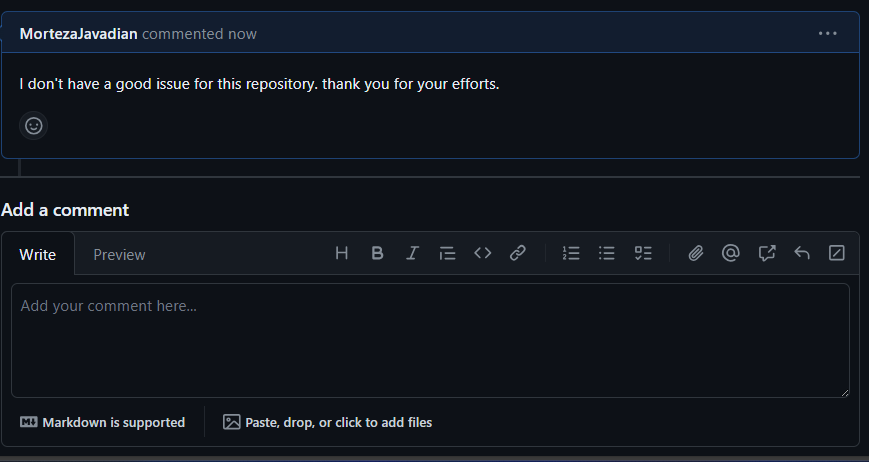
\includegraphics[width=0.8\textwidth]{Screenshot.png}
		\caption{This picture is my issues}
	\end{figure}

	\subsection{README}
	
	\begin{figure}[h]
		\centering
		
\includegraphics[width=0.8\textwidth]{Screenshot2.png}
		\caption{This picture is my README}
	\end{figure}

	My github repository of final Assignment:
	
	https://github.com/MortezaJavadian/Final-Assignment
	
\end{document}